\section{Benutzeroberfläche}

Beim Starten der Applikation öffnet sich das User Interface des Simulators auf dem die Funktionen des PICs nachvollzogen werden können.

\begin{figure}[h]
\centering
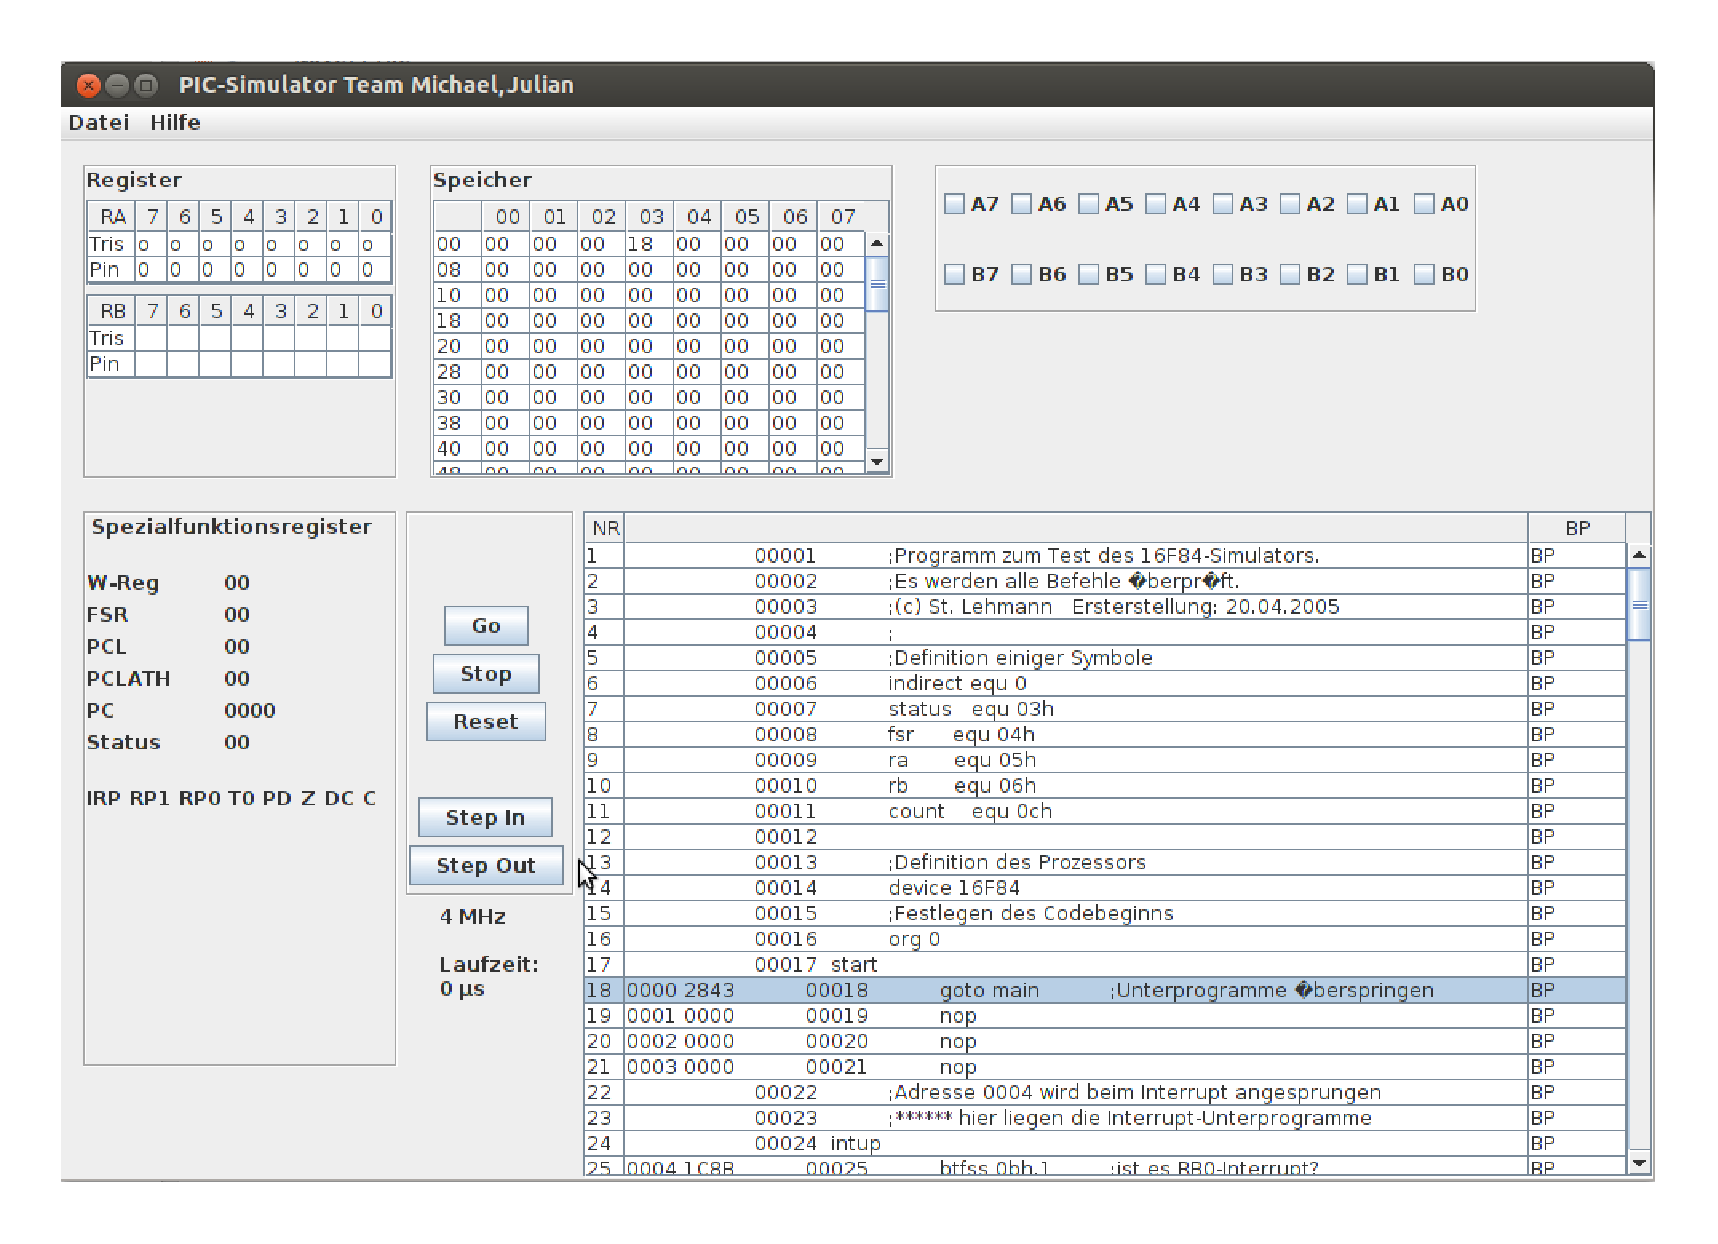
\includegraphics[scale=0.4]{Bilder/GUI.pdf}
\caption{GUI}
\end{figure}
\newpage

\noindent Über „Datei“ und „Datei öffnen“ lassen sich Quellcode-Dateien öffnen. In die Dateiauswahl ist ein Dateifilter integriert der ausschließlich .LST-Dateien anzeigt.

\begin{figure}[h]
\centering
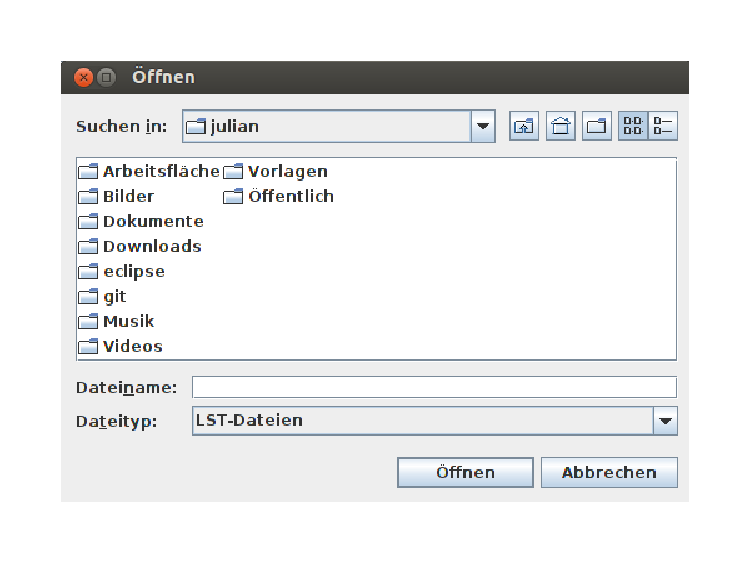
\includegraphics[scale=0.7]{Bilder/Offnen.pdf}
\caption{Datei öffnen}
\end{figure}

\noindent Mit den Buttons "Step-In", "Step-Out", "Go", "Stop" und "Reset" lässt sich der Simulationsablauf steuern. Mit Step-In und Step-Out lässt sich jeweils nur ein Programmschritt ausführen, mit Go wird das Programm komplett abgearbeitet. Mit Stop stoppt der Simulationsvorgang und mit Reset wird er komplett zurückgesetzt.

\begin{figure}[h]
\centering
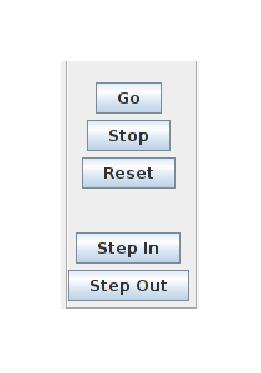
\includegraphics[scale=0.5]{Bilder/Buttons.pdf}
\caption{Kontroll-Buttons}
\end{figure}

Die Register werden in der linken oberen Ecke des User Interfaces angezeigt. Die werte des Spezialfunktionsregister wird darunter dargestellt. Die  Darstellung der Werte erfolgt im Hexadezimalsystem.

\begin{figure}[h]
\centering
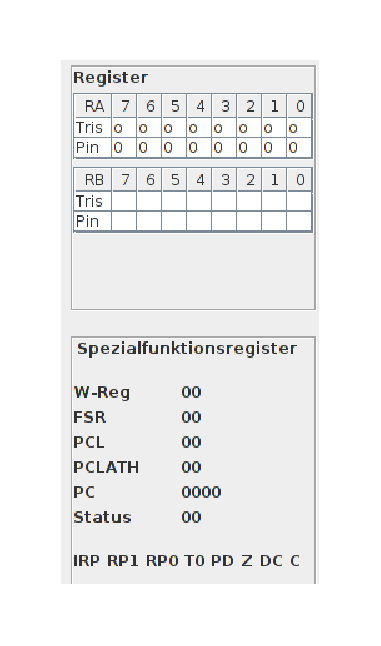
\includegraphics[scale=0.5]{Bilder/Register.pdf}
\caption{Register und Spezialfunktionsregister}
\end{figure}

Die Speicherinhalte werden in Form einer Tabelle am oberen Rand des User Interfaces dargestellt. Die Werte werden im Hexadezimalsystem wiedergegeben. 


\noindent In der rechten unteren Ecke wir der Quelltext des zu simulierenden Programmes angezeigt. Dieser wir wie beschrieben über "Datei öffnen" in die Tabelle geschrieben.

\begin{figure}[h]
\centering
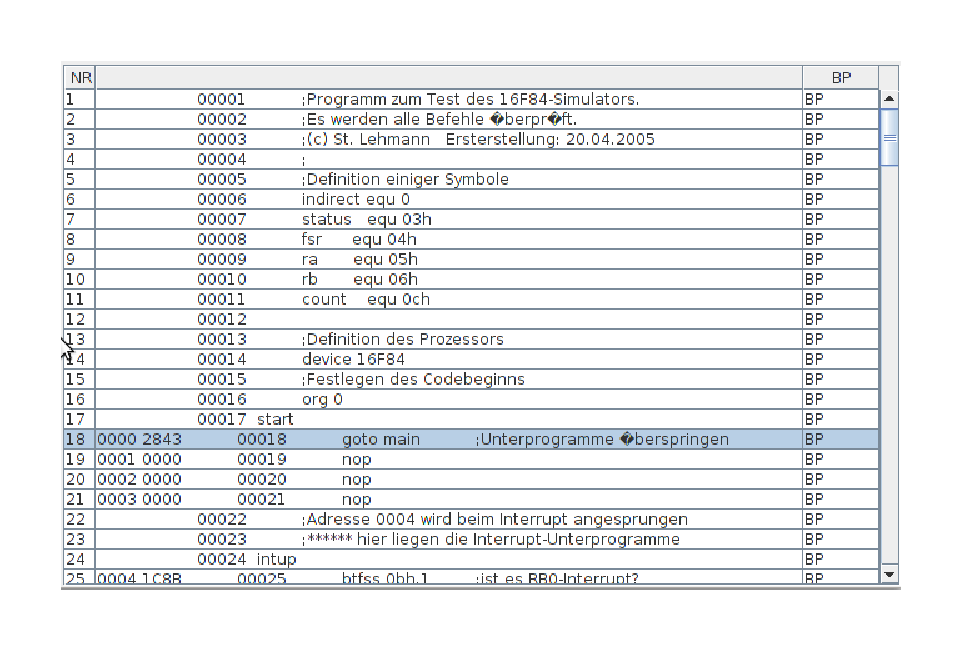
\includegraphics[scale=0.5]{Bilder/Text.pdf}
\caption{Textfeld für den Quelltext}
\end{figure}